\documentclass[bigger]{beamer}

\setbeamertemplate{bibliography item}[text]

\usepackage[utf8]{inputenc}
\usepackage[T1]{fontenc}
\usepackage{fixltx2e}
\usepackage{graphicx}
\usepackage{longtable}
\usepackage{float}
\usepackage{wrapfig}
\usepackage[normalem]{ulem}
\usepackage{textcomp}
\usepackage{marvosym}
\usepackage{wasysym}
\usepackage{latexsym}
\usepackage{amssymb}
\usepackage{amstext}
\usepackage{hyperref}
\usepackage{natbib}
% amsmath and amssymb packages, useful for mathematical formulas and symbols
\usepackage{amsmath,amssymb}
\usepackage{textcomp,marvosym}
\newcommand{\R}{\texttt{R} }
\newcommand{\code}[1]{{\texttt{#1}}}
\newcommand{\Rfunction}[1]{{\texttt{#1}}}
\newcommand{\Robject}[1]{{\texttt{#1}}}
\newcommand{\Rpackage}[1]{{\mbox{\normalfont\textsf{#1}}}}
\newcommand{\email}[1]{\href{mailto:#1}{\normalfont\texttt{#1}}}

%% Include all macros below

\newcommand{\lorem}{{\bf LOREM}}
\newcommand{\ipsum}{{\bf IPSUM}}

\newcommand{\bx}{\mathbf{x}}
\newcommand{\bv}{\mathbf{v}}
\newcommand{\bp}{\mathbf{p}}
\newcommand{\bq}{\mathbf{q}}
\newcommand{\by}{\mathbf{y}}

\newcommand{\bbR}{\mathbb{R}}
\newcommand{\bbN}{\mathbb{N}}

\newcommand{\bxi}{\bm{\xi}}
\newcommand{\bal}{\bm{\alpha}}
\newcommand{\bth}{\bm{\theta}}

%% END MACROS SECTION


%% Additional packages
\usepackage{bm}

%% colors
\definecolor{Red}{rgb}{0.7,0,0}
\definecolor{Blue}{rgb}{0,0,0.8}

\usepackage{hyperref}
\usepackage{breakurl}
\hypersetup{%
  pdfauthor={Laurent Gatto},%
  pdfusetitle,
  bookmarks = {true},
  bookmarksnumbered = {true},
  bookmarksopen = {true},
  bookmarksopenlevel = 2,
  unicode = {true},
  breaklinks = {false},
  hyperindex = {true},
  colorlinks = {true},
  linktocpage = {true},
  plainpages = {false},
  linkcolor = {Blue},
  citecolor = {Blue},
  urlcolor = {Red},
  pdfstartview = {Fit},
  pdfpagemode = {UseOutlines},
  pdfview = {XYZ null null null}
}
%----------------------------------------------------------------------------------------
%	TITLE PAGE
%----------------------------------------------------------------------------------------

%\author{L. Breckels*, K.S. Lilley and L. Gatto, \\
%University of Cambridge}
\title{Interactive visualisation of spatial proteomics data}
\author{L. Breckels and L. Gatto}
\institute{
University of Cambridge, UK | de Duve Institute, Belgium\\
lms79@cam.ac.uk | laurent.gatto@uclouvain.be\\
\bigskip
Slides:  
\includegraphics[height=3mm]{./Figures/zenodo1927886.png}\\
\url{https://zenodo.org/record/1927886}}

\date{\small EuroBioC 2018, 6-7th December 2018}




\begin{document}

\maketitle


%----------------------------------------------------------------------------------------
%	SLIDE 1 ---- Protein localisation - why?
%----------------------------------------------------------------------------------------

\section{Spatial proteomics}

\begin{frame}{Cell organisation}
  \begin{columns}[t]
    \begin{column}[T]{0.5\textwidth}
      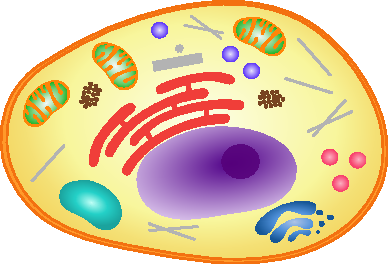
\includegraphics[width=1\linewidth]{Figures/cell.pdf}
    \end{column}
    \begin{column}[T]{0.5\textwidth}
       \begin{itemize}
         \item \scriptsize Proteins are spatially organised according to function
        \item Significant correlation between disease classes and sub-cellular localisations
        \item Abnormal protein localisation leading to the loss of functional effects in diseases
       \end{itemize}
           \end{column}
  \end{columns}
  \bigskip
\textbf{\textcolor{Blue}{Spatial proteomics}} is the systematic
    study of protein localisations.
\end{frame}


%----------------------------------------------------------------------------------------
%	SLIDE 2 ---- Localisation Maps
%----------------------------------------------------------------------------------------

\section{Global localisation maps}

\begin{frame}{Localisation maps from quantitative proteomics}
\bigskip
      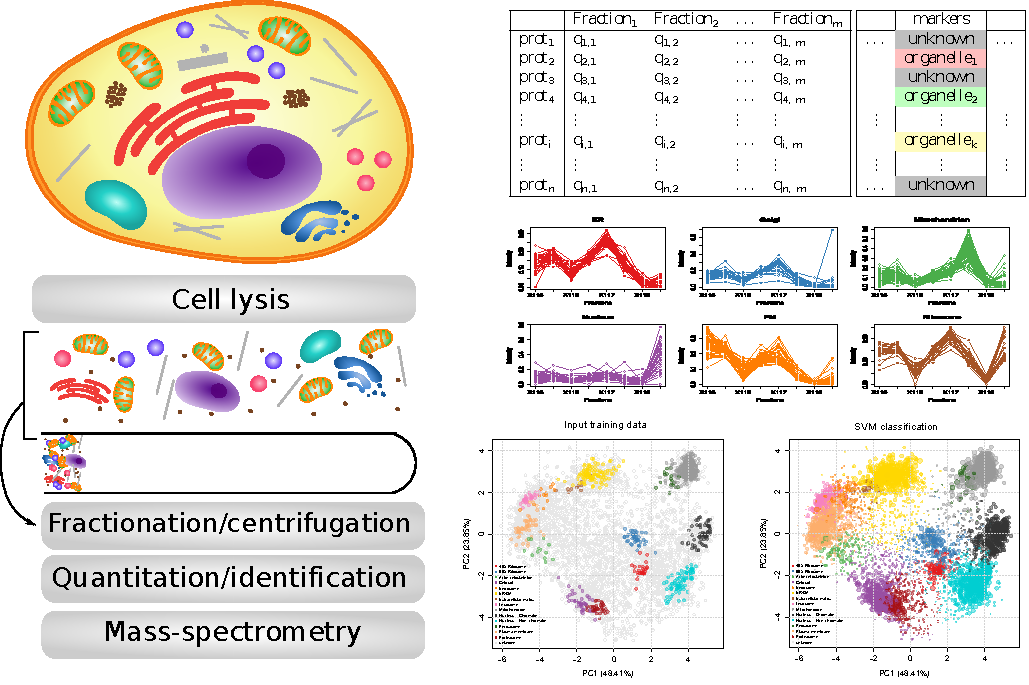
\includegraphics[width=1\linewidth]{Figures/lopit-new.pdf}
       \begin{center}
       \footnotesize{Goal: to pinpoint the sub-cellular localisation of proteins}
       \end{center}

\end{frame}




%----------------------------------------------------------------------------------------
%	SLIDE 3 ---- A complete suite of software
%----------------------------------------------------------------------------------------

\begin{frame}{A synergistic framework}
  \begin{block} \large \textcolor{Blue}{Data analysis and machine learning}
  \begin{itemize}
  \item MSnbase and pRoloc - dedicated packages providing robust
  and reproducible tools
   \end{itemize}
  \end{block}

  \begin{block} \large \textcolor{Blue}{Data visualisation}
    \begin{itemize}
    \item pRolocGUI - interactive visualisation and data mining
    \item User driven: essential to transfer of findings easily between
    programmatic and graphical interfaces
    \end{itemize}
  \end{block}
\end{frame}

%----------------------------------------------------------------------------------------
%	SLIDE 4 ---- The pRolocGUI package
%----------------------------------------------------------------------------------------

\begin{frame}{The pRolocGUI package}
 \begin{small}
\begin{enumerate}
\item The \textit{main app} - for exploratory data analysis and features a
searchable, clickable and zoomable PCA plot
\item The \textit{comparison app} - for examining two replicate experiments,
or two experiments from different conditions etc
\item The \textit{aggregation app} - allows one to compare the effects of
feature aggregation, for example, when combining peptides to proteins
\item The \textit{classify app} - useful for viewing the sub-cellular class
predictions output from a supervised machine learning analysis
\end{enumerate}
\end{small}
\end{frame}


%% %----------------------------------------------------------------------------------------
%% %	SLIDE 5 ---- The main application
%% %----------------------------------------------------------------------------------------

%% \begin{frame}{The main application}
%% \smallskip
%%   \begin{small} \textbf{Use case:} hyperLOPIT on mouse embryonic stem cells
%%   \end{small}
%%   \begin{figure}
%%     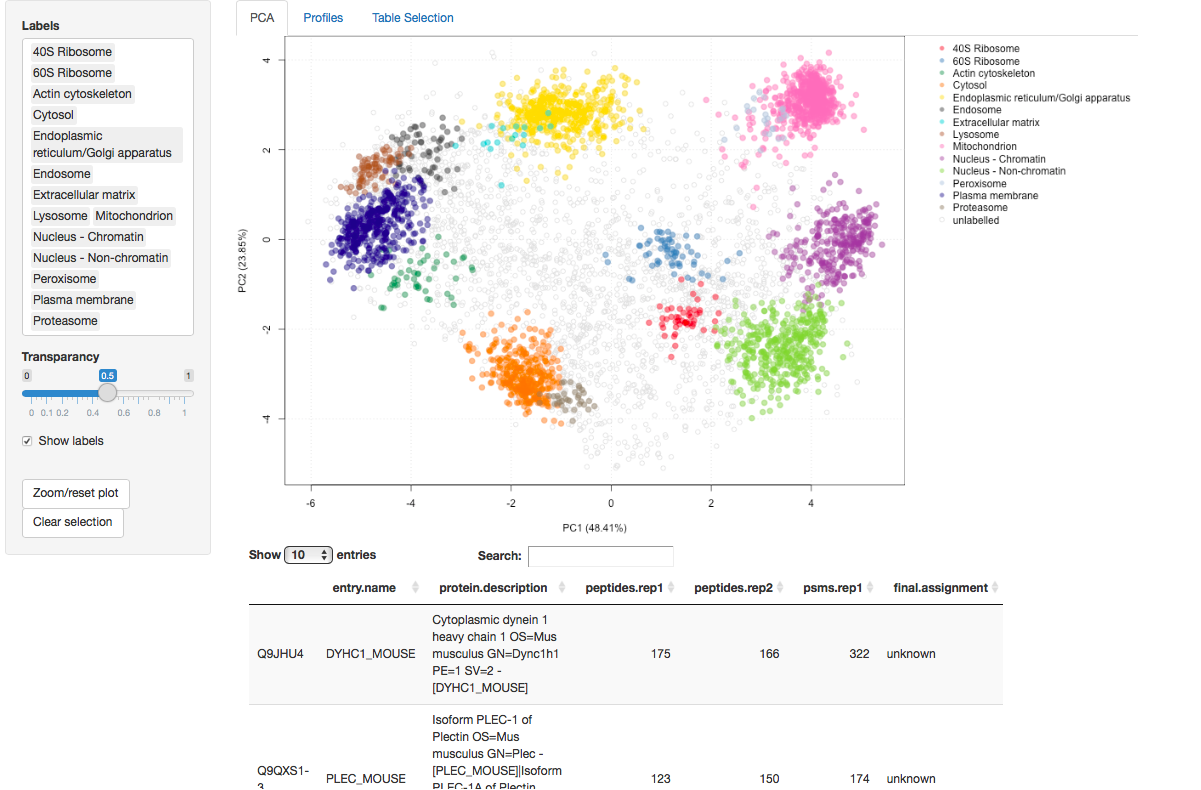
\includegraphics[width=1\linewidth]{Figures/main-app.png}
%%   \end{figure}
%% \end{frame}


%% %----------------------------------------------------------------------------------------
%% %	SLIDE 6 ---- The aggregation application
%% %----------------------------------------------------------------------------------------

%% \begin{frame}{The aggregation application}
%% \smallskip
%%   \begin{small} \textbf{Use case:} Protein and peptide localisation
%%   \end{small}
%%   \begin{figure}
%%     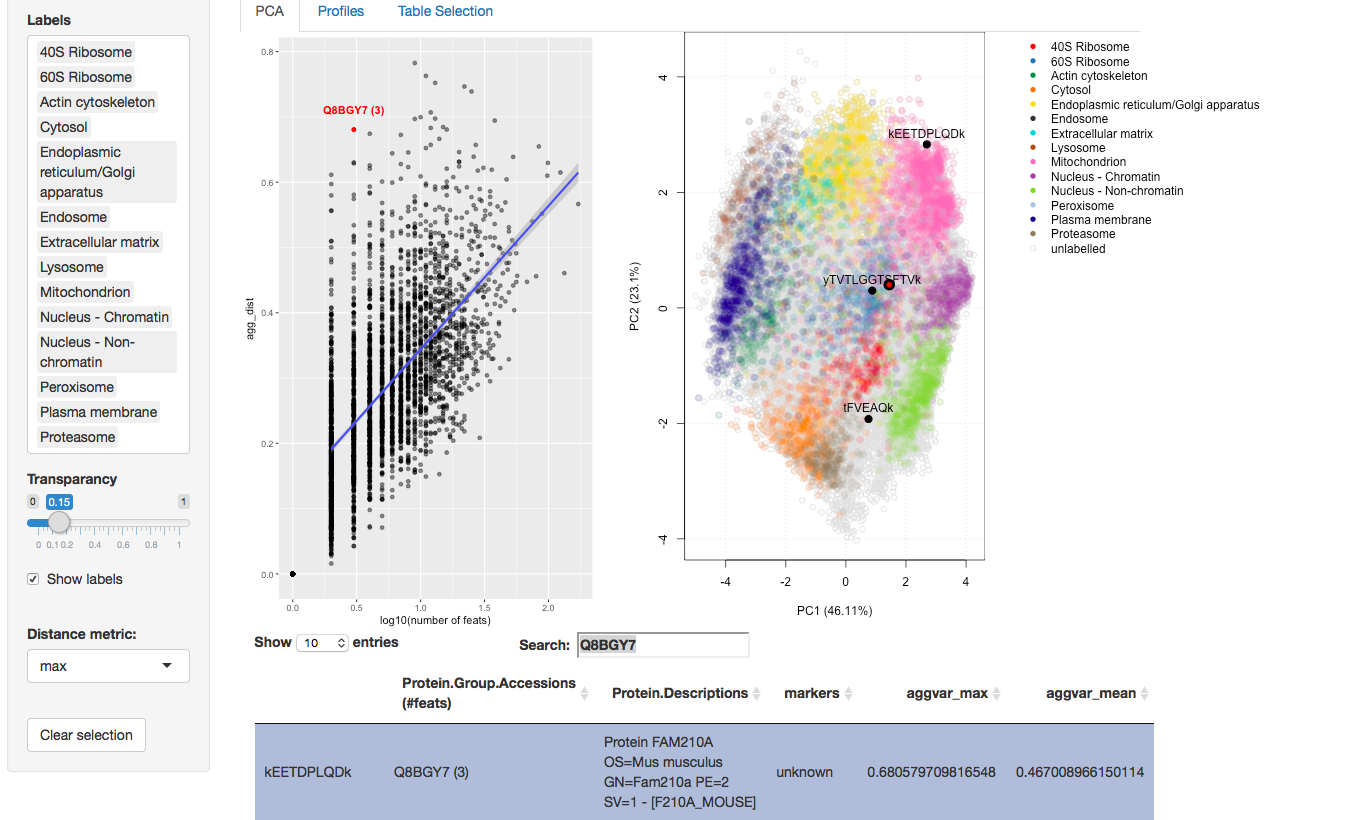
\includegraphics[width=1\linewidth]{Figures/agg-app.png}
%%   \end{figure}
%% \end{frame}

%% %----------------------------------------------------------------------------------------
%% %	SLIDE 7 ---- The classify application
%% %----------------------------------------------------------------------------------------

%% \begin{frame}{The classify application}
%% \smallskip
%%   \begin{small} \textbf{Use case:} Setting thresholds for protein location by SVM
%%   \end{small}
%%   \begin{figure}
%%     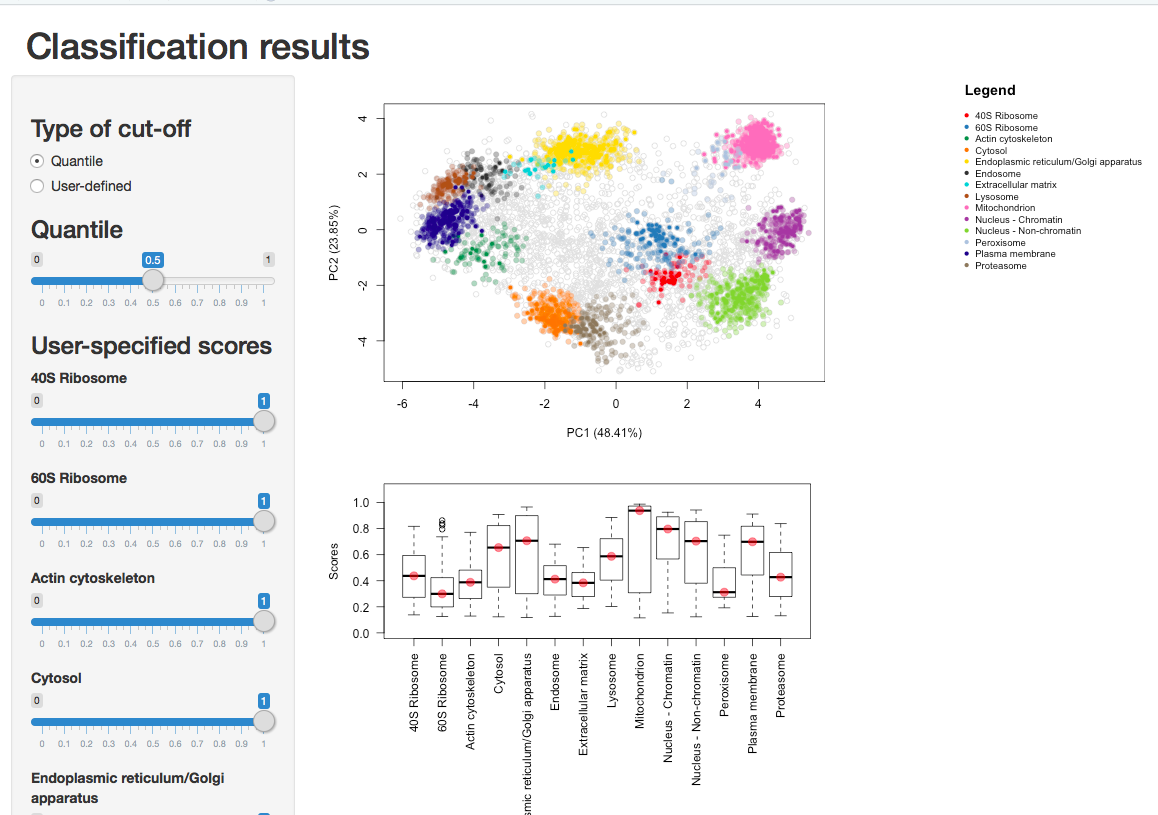
\includegraphics[width=1\linewidth]{Figures/classify-app.png}
%%   \end{figure}
%% \end{frame}

%% %----------------------------------------------------------------------------------------
%% %	SLIDE 8 ---- The comparison application
%% %----------------------------------------------------------------------------------------

%% \begin{frame}{The comparison application}
%% \smallskip
%%   \begin{small} \textbf{Use case:} hyperLOPIT on THP1 monocytic cancer cells after 12 hours LPS stimualtion
%%   \end{small}
%%   \begin{figure}
%%     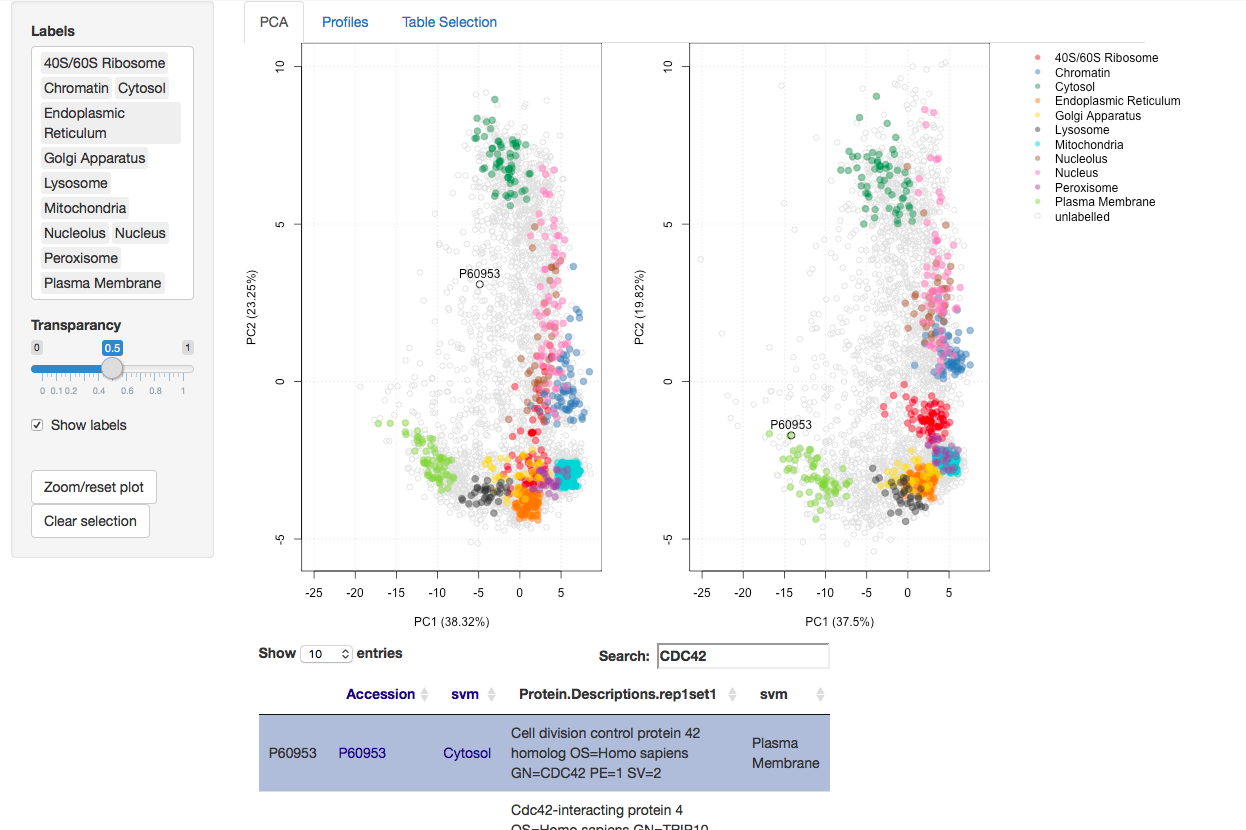
\includegraphics[width=1\linewidth]{Figures/compare-app.png}
%%   \end{figure}
%% \end{frame}


%----------------------------------------------------------------------------------------
%	SLIDE 8 ---- EXTRA SLIDES
%----------------------------------------------------------------------------------------

\begin{frame}{Main app - Example 1: TRAPP complex}
\smallskip
\footnotesize {
  \begin{itemize}
  \item TRAPP complex (trafficking protein particle complex)
  \item Multi-localised: involved in trafficking between ER/GA and PM
  \item Note: one protein sits away, investigation shows it has a separate  role
  as an activator of NF-kappa-B through increased phosphorlyation
  \end{itemize}
  }
  \begin{figure}
    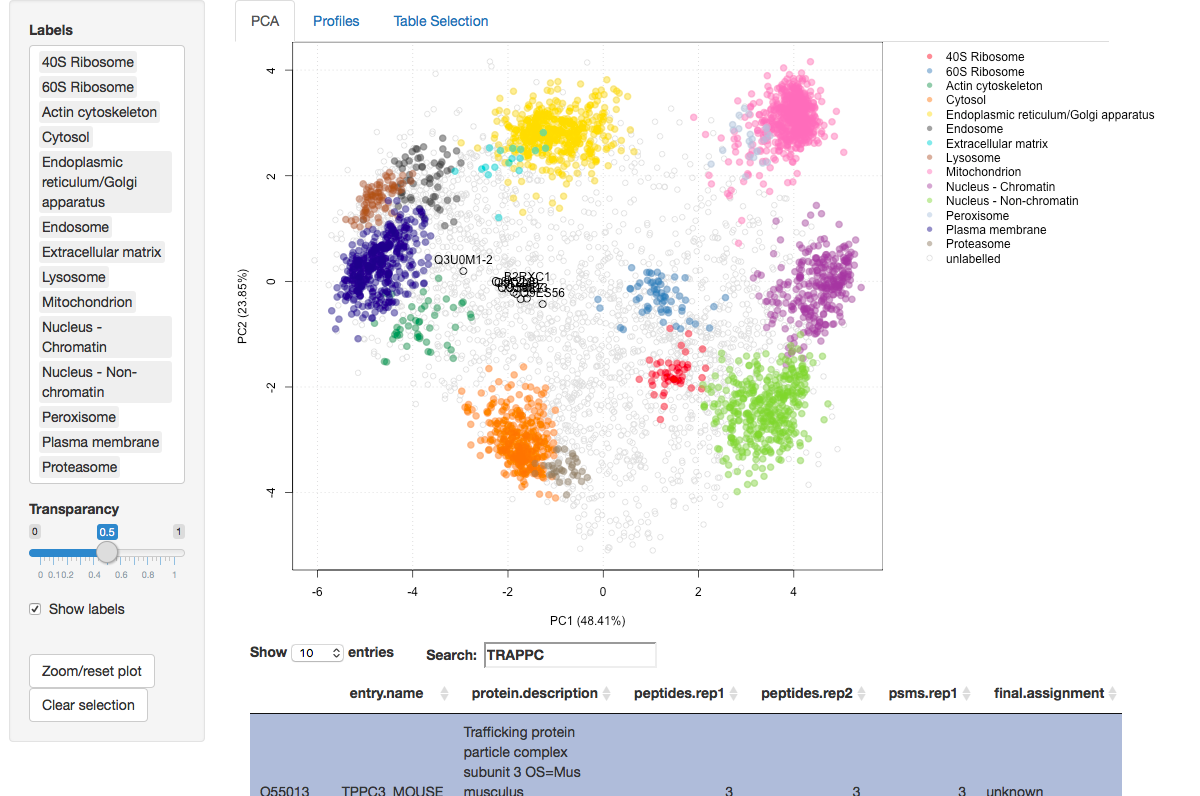
\includegraphics[width=.5\linewidth]{Figures/demo1-trapp-pca.png}
    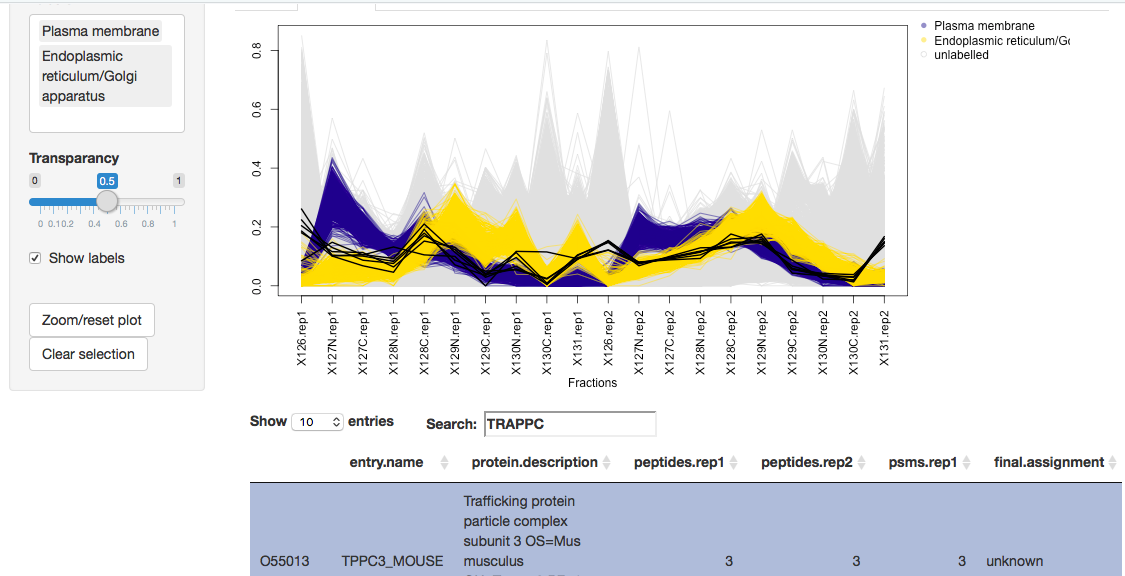
\includegraphics[width=.5\linewidth]{Figures/demo1-trapp-profiles.png}
  \end{figure}
\end{frame}


\begin{frame}{Main app - Example 2: EIF3 complex}
\smallskip
\footnotesize {
  \begin{itemize}
  \item Eukaryotic initiation factor 3 (eIF3) is a multiprotein complex that functions during the initiation phase of translation
  \item eIF3 stimulates nearly all steps of translation initiation
  \item location and profiles highly correlated -> well characterised complex
  \end{itemize}
  }
  \begin{figure}
    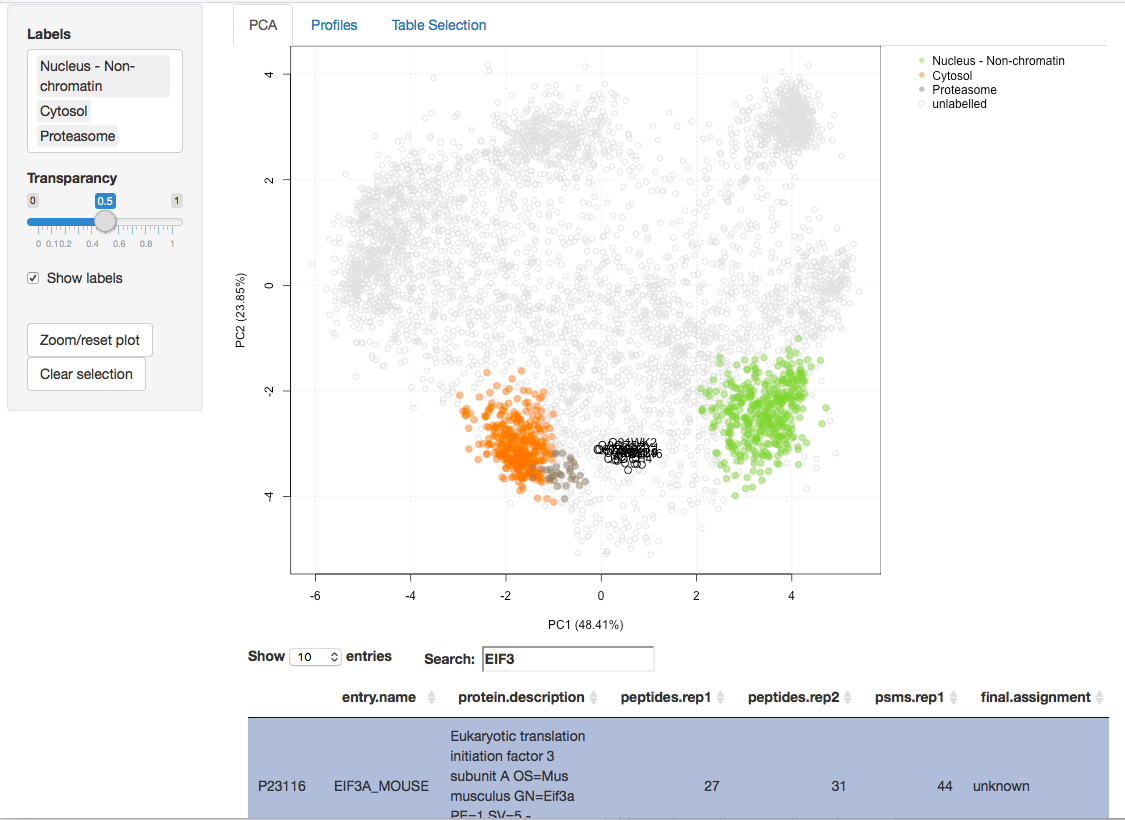
\includegraphics[width=.5\linewidth]{Figures/demo2-eif3-pca.png}
    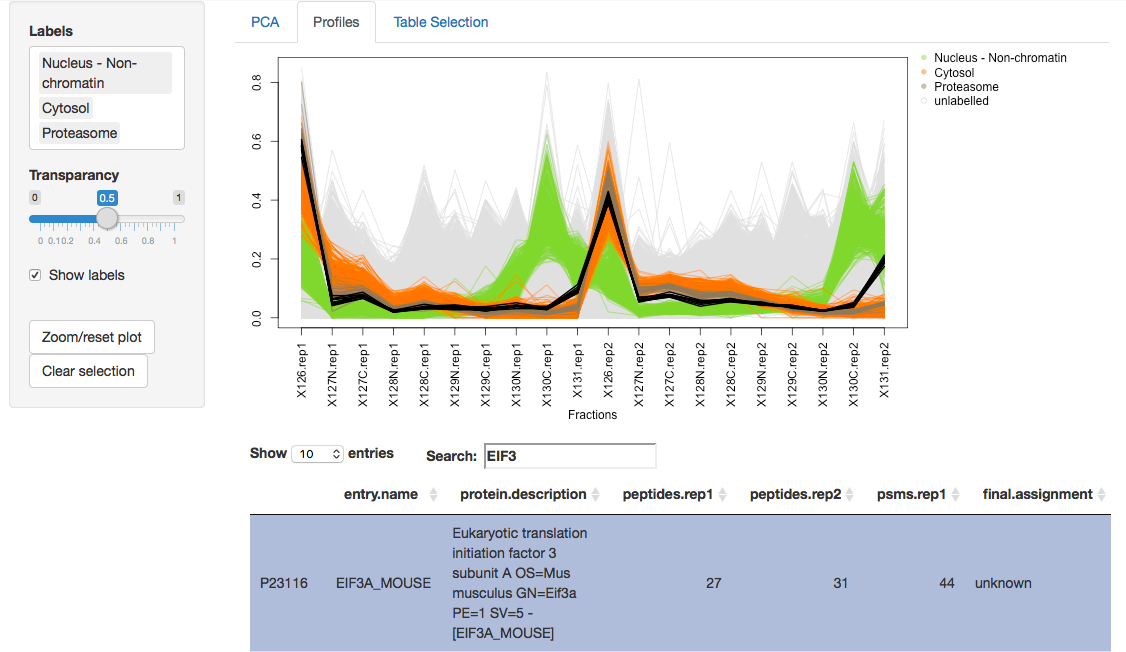
\includegraphics[width=.5\linewidth]{Figures/demo2-eif3-profiles.png}
  \end{figure}
\end{frame}



\begin{frame}{Main app - Example 3: Visualisation of many complexes}
\smallskip
\footnotesize {
  \begin{itemize}
  \item The application is well suited to visualisation of multiple organelles/complexes/sub-cellular niches
  \item The handy drop down menu allows one to easily click on/off compartments - avoid
  the regeneration of multiple plots etc.
  \end{itemize}
  }
  \begin{figure}
    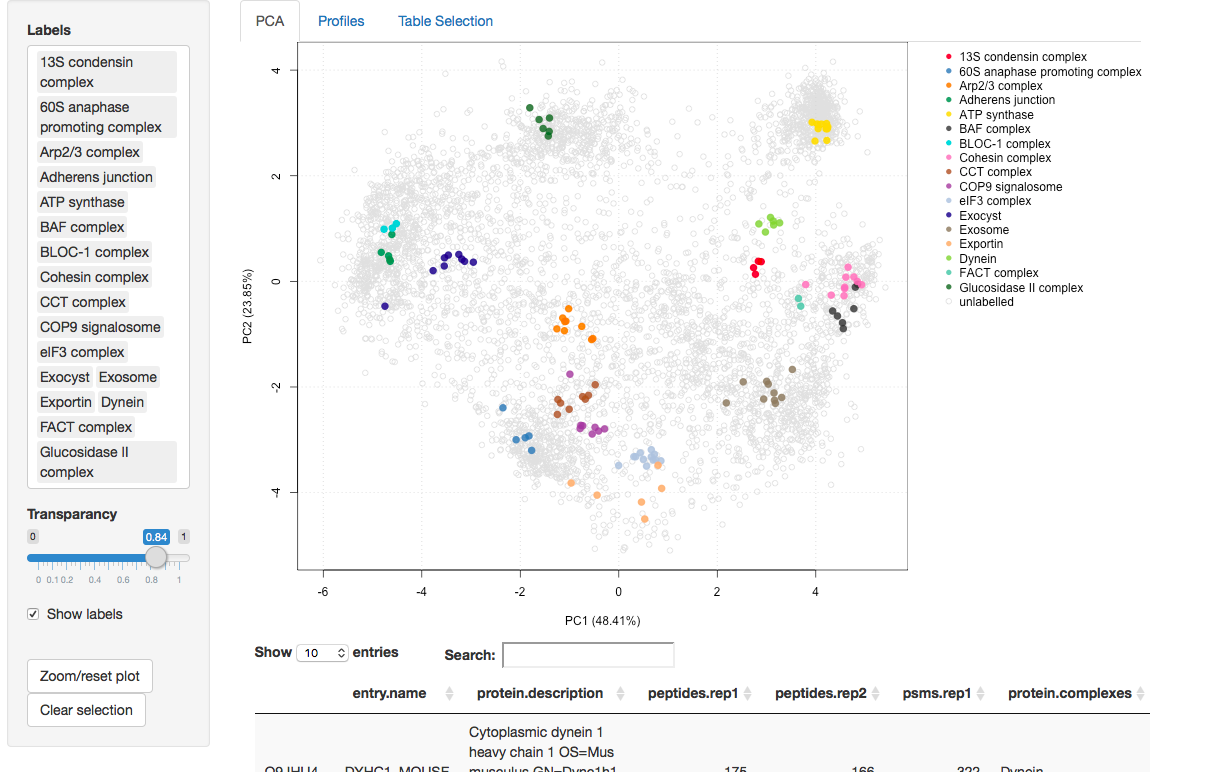
\includegraphics[width=.7\linewidth]{Figures/demo3-protein-complexes.png}
  \end{figure}
\end{frame}


\begin{frame}{Aggregation app - Example 4: Protein FAM210A}
\smallskip
\footnotesize {
  \begin{itemize}
  \item This is an interesting protein found from looking at the outliers of the aggvar plot on the LHS
  \item 3 PSMs available for quantitation all with very different localisations on the plot
  \item Not much was known about this proteins function until this year (see http://www.pnas.org/content/115/16/E3759)
  \item Is is expressed in muscle mitochondria and cytoplasm
  \item Thought to strongly influence the structure and strength of both muscle and bone and a new target for osteoporosis
  \end{itemize}
  }
  \begin{figure}
    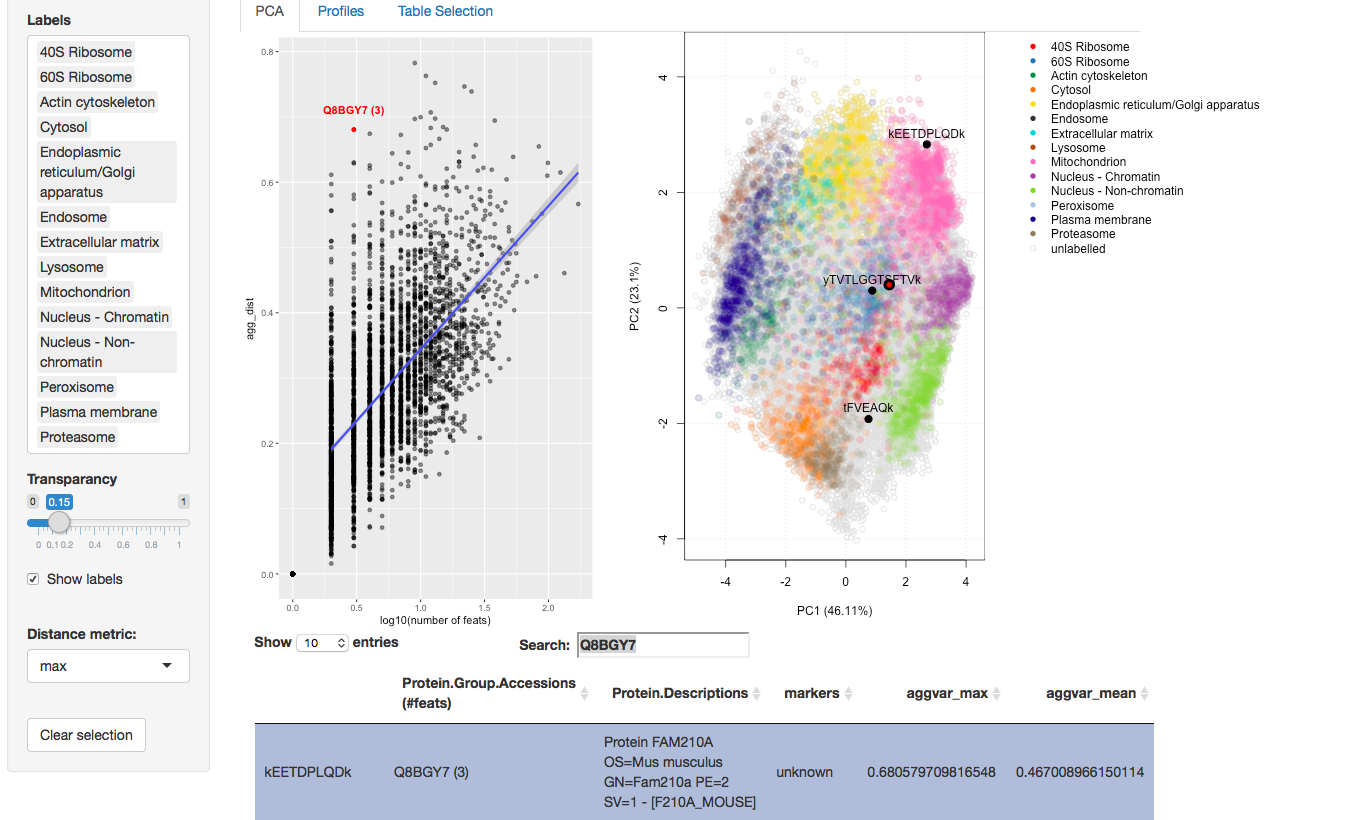
\includegraphics[height=.4\linewidth]{Figures/agg-app.png}
  \end{figure}
\end{frame}


\begin{frame}{Classify app - Example 5: Visualisation of ML results}
\smallskip
\footnotesize {
  \begin{itemize}
  \item Load the SVM classification results from the mouse stem cell dataset
  \item Explain how users set thresholds
  \item See the effects on classifictaion of setting thresholds
    \end{itemize}
  }
  \begin{figure}
      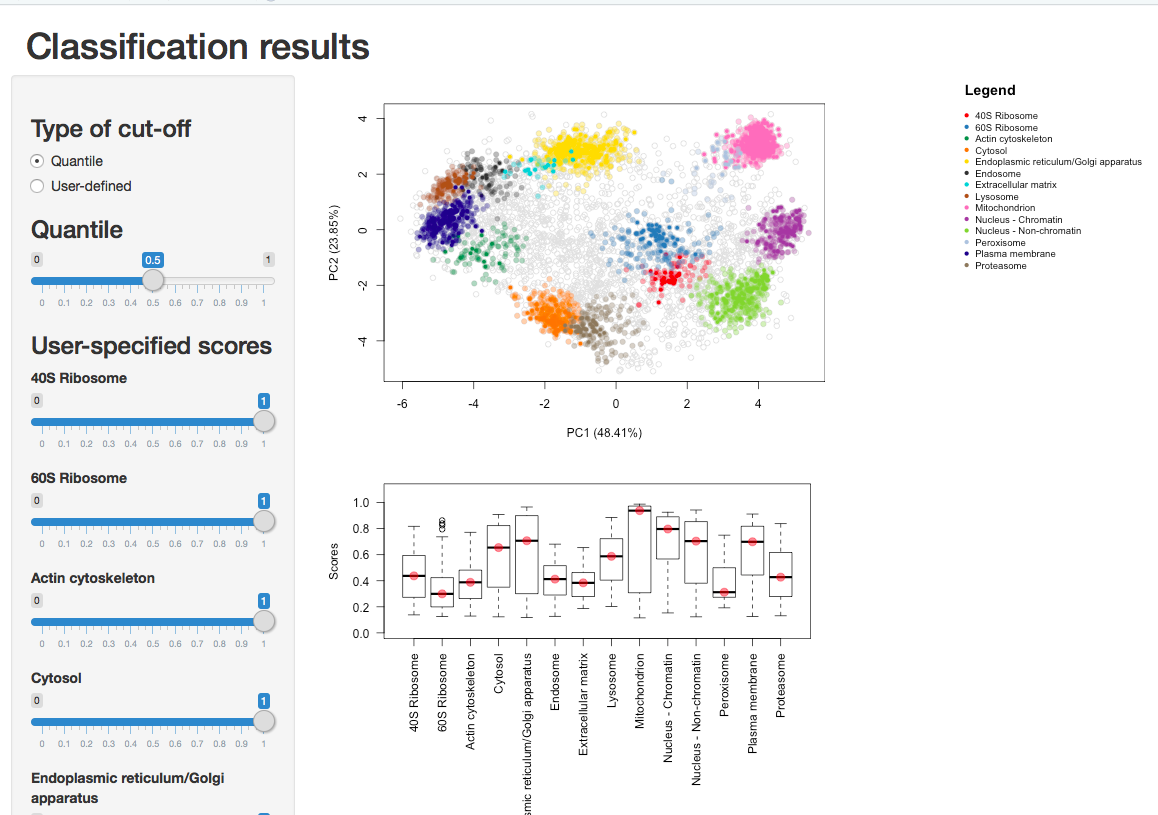
\includegraphics[width=.7\linewidth]{Figures/classify-app.png}
  \end{figure}
\end{frame}


\begin{frame}{Compare app - Example 6: Human THP data (a monocytic cancer cell line)}
\smallskip
\footnotesize {
  \begin{itemize}
  \item hyperLOPIT experiment on a THP1 cells, 3 x 20 fractions (two 10 plex TMT each replicate)
  \item Unstimulated (LHS) and cells treated with Lipopolysaccharide (LPS) (12 hrs stimulation) (RHS)
  \item Many proteins re-localise after 12 hours LPS stimulations
  \item Example 1 - CDC42. In active state binds to a variety of effector proteins to regulate cellular responses at the plasma membrane (PM)
  \item Example 2 - RABs. Another GTPase regulates membrane trafficking to regulate cellular responses at the plasma membrane (PM) (RAB32 --->  GA to ER, RAB12 --->  PM to GA, RAB6B --->  GA to PM)
    \end{itemize}
  }
\end{frame}


\begin{frame}{Compare app - Example 6: Human THP data (a monocytic cancer cell line)}
  \begin{figure}
      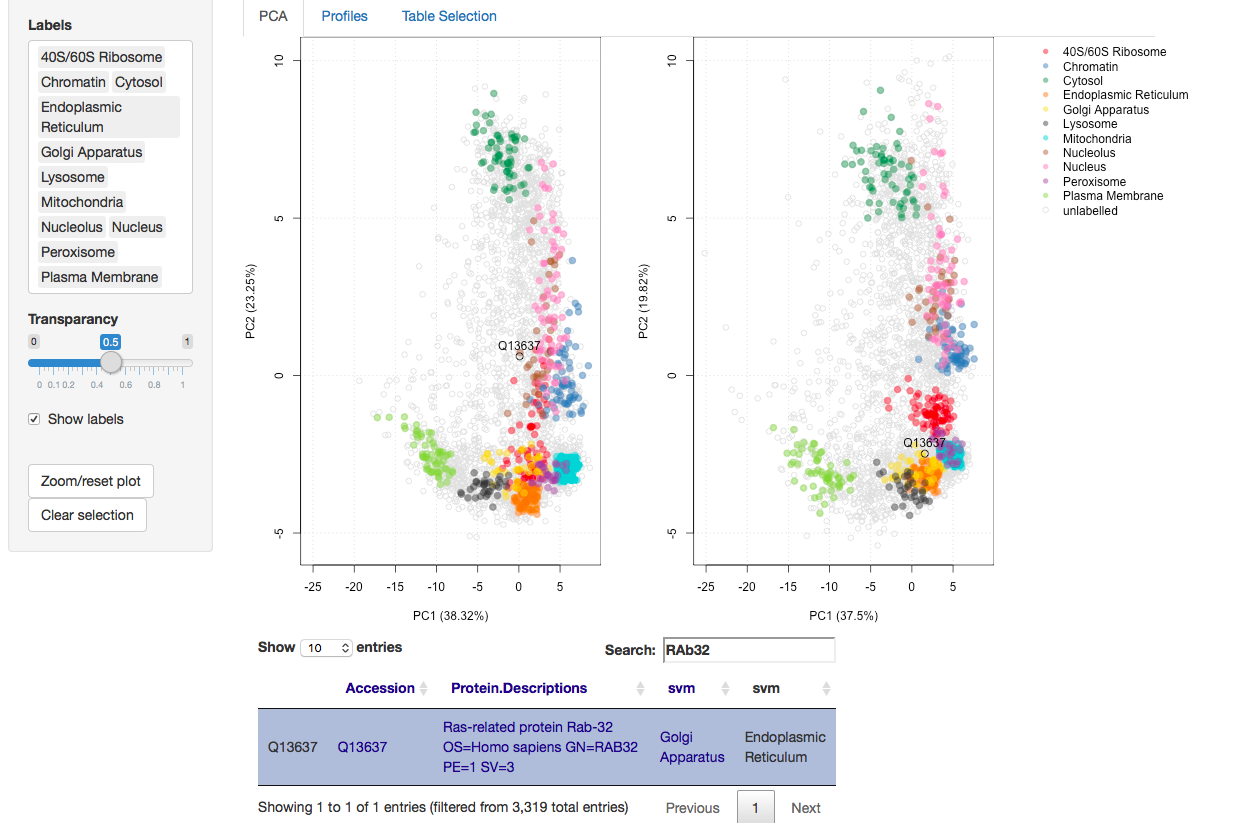
\includegraphics[width=1\linewidth]{Figures/demo6b-rab32-pca.png}
  \end{figure}
\end{frame}


%----------------------------------------------------------------------------------------
%	Acknowledgements
%----------------------------------------------------------------------------------------
  \begin{frame}

   \begin{block}{Software}
     \vspace{.1cm}
     Infrastructure: \Rpackage{MSnbase} \newline
     ML: \Rpackage{pRoloc} \newline
     Visualisation: \Rpackage{pRolocGUI} \newline
     Data: \Rpackage{pRolocdata}.
    \vspace{.2cm}
  \end{block}

  \begin{block}{Acknowledgements}
    \begin{itemize}
    \item Prof. Kathryn Lilley (Cambridge Centre for Proteomics)
    \item Funding: BBSRC
    \end{itemize}
  \end{block}

  \begin{block}{Slides}
    \begin{itemize}
    \item \url{https://zenodo.org/record/1927886}
    \end{itemize}
  \end{block}

  \end{frame}



\end{document}
